\documentclass[8pt]{article}
\usepackage[margin=0.25in]{geometry}
\usepackage{amsmath, amssymb}
\usepackage{multicol}
\usepackage{graphicx} % Added to allow image insertion
\usepackage{titlesec} % Added to squeeze header spacing

\setlength{\columnsep}{0.7cm}
\setlength{\parindent}{0in}

% --- Squeezing Space ---
\linespread{0.65} % Reduces global vertical line spacing
% Format: \titlespacing*{command}{left}{before-sep}{after-sep}
\titlespacing*{\section}{0pt}{2pt}{1pt}
\titlespacing*{\subsection}{0pt}{2pt}{1pt}
% -----------------------

\date{}

\begin{document}
\large ENGR 232 Exam 1 Notesheet \hfill Sean Balbale \hfill March 2026 \vspace{0.1cm}
\hrule
\vspace{0.1cm}

\begin{multicols*}{2}

  \section*{Chapter 2: Atomic Structure \& Bonding}
  \subsection*{Key Equations}
  \textbf{Average Atomic Weight:} \( A_{avg} = \sum f_{i} A_{i} \) \\
  (\( A_{avg} \): average atomic wt, \( f_{i} \): fraction of occurrence, \( A_{i} \): atomic wt of isotope \( i \)) \\

  \textbf{Force of Attraction:} \( F_{A} = \frac{|Z_{1} Z_{2}| e^{2}}{4 \pi \epsilon_{0} r^{2}} \) \\
  (\( F_{A} \): attractive force, \( Z_{1}, Z_{2} \): ion valences, \( r \): interatomic distance) \\
  Constants: \( e = 1.602 \times 10^{-19} \text{ C} \) (electron charge), \( \epsilon_{0} = 8.85 \times 10^{-12} \text{ F/m} \) (permittivity of vacuum). \\

  \textbf{Percent Ionic Character (\%IC):} \\
  \( \%IC = \left( 1 - e^{-0.25(X_{A} - X_{B})^{2}} \right) \times 100 \) \\
  (\( X_{A}, X_{B} \): electronegativities of elements A and B)

  \subsection*{Concepts}
  \textbf{Bohr Model:} Electrons orbit a central nucleus in discrete energy levels. \\
  \begin{center}
    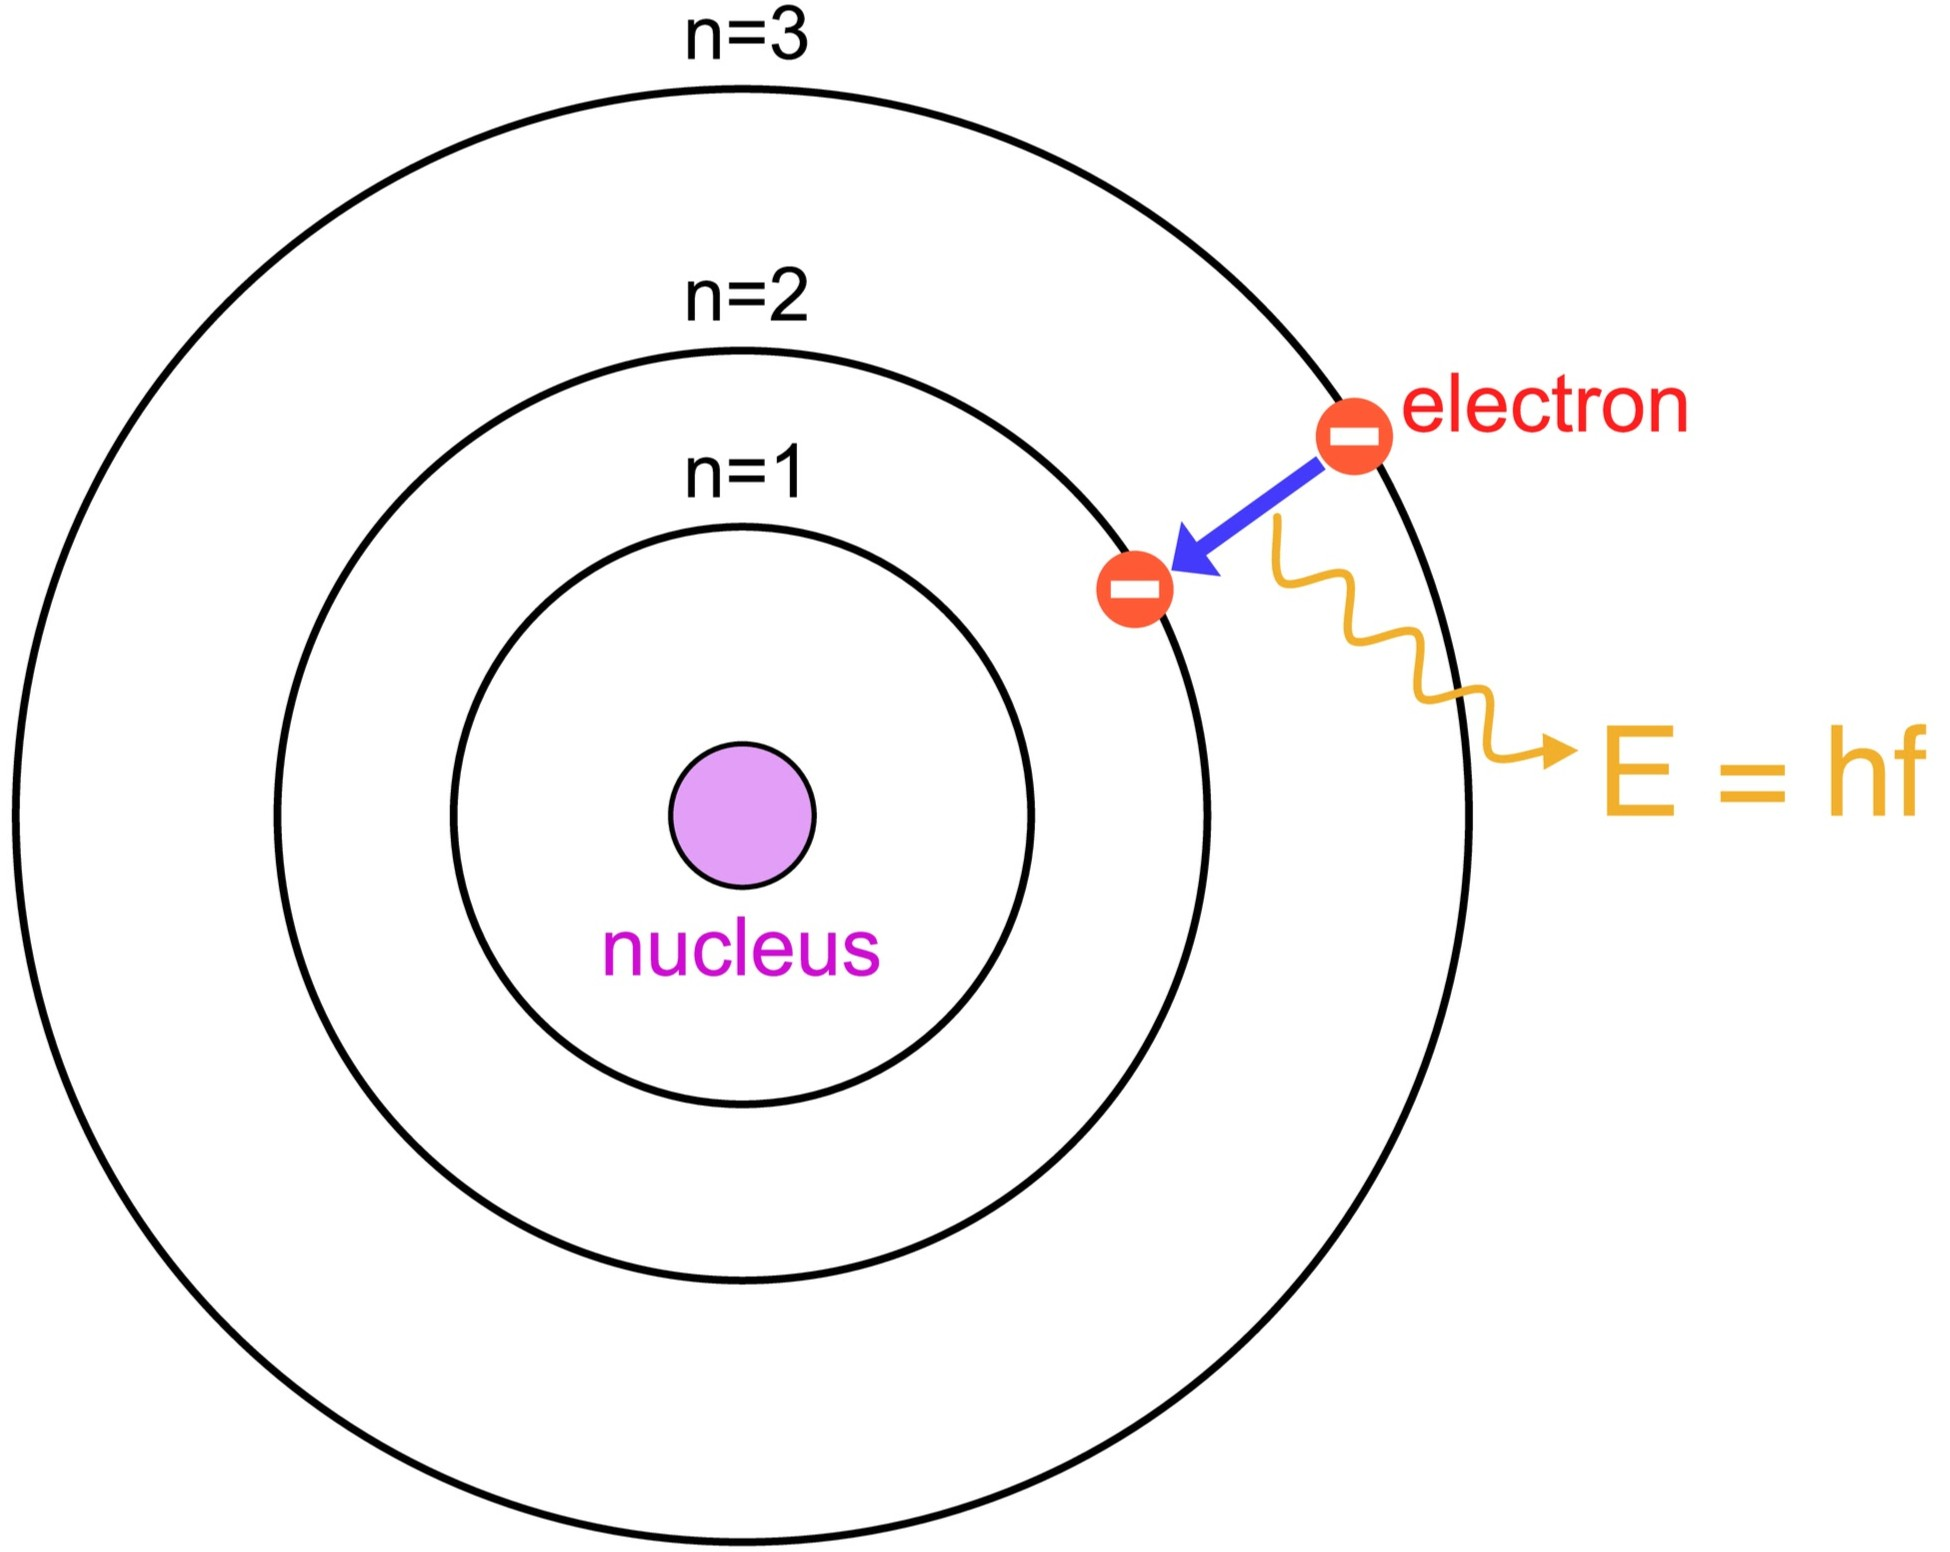
\includegraphics[width=0.55\linewidth]{bhormodel.jpg}
  \end{center}
  \textbf{Bonding:} Ionic (electron transfer), Covalent (electron sharing), Metallic (sea of delocalized electrons).

  \subsection*{Example: Force of Attraction}
  Calculate force between \( K^+ \) (\( Z_1=+1 \)) and \( I^- \) (\( Z_2=-1 \)) separated by \( 0.314 \) nm.\\
  \( r = 0.314 \times 10^{-9} \text{ m} \). \\
  \( F_{A} = \frac{|(1)(-1)| (1.602 \times 10^{-19})^{2}}{4 \pi (8.85 \times 10^{-12}) (0.314 \times 10^{-9})^{2}} = 2.33 \times 10^{-9} \text{ N} \)

  \section*{Chapter 3: Crystal Structures}
  \subsection*{Key Equations \& Geometry}
  \textbf{SC Edge Length:} \( a = 2R \), \( n = 1 \) atom/cell. \\
  \textbf{BCC Edge Length:} \( a = \frac{4R}{\sqrt{3}} \), \( n = 2 \) atoms/cell. \\
  \textbf{FCC Edge Length:} \( a = 2R\sqrt{2} \), \( n = 4 \) atoms/cell. \\
  (\( a \): unit cell edge length, \( R \): atomic radius, \( n \): atoms per unit cell) \\

  \textbf{Atomic Packing Factor (APF):} Fraction of solid sphere vol. \\
  \( APF = \frac{\text{Vol. of atoms}}{\text{Vol. of unit cell}} = \frac{n (\frac{4}{3}\pi R^3)}{a^3} \) \\
  (SC = 0.52, BCC = 0.68, FCC = 0.74) \\

  \textbf{Unit Cell Volume:} \( V_{c} = a^{3} \) \\
  \textbf{Theoretical Density:} \( \rho = \frac{n A}{V_{c} N_{A}} \) \\
  Constant: \( N_{A} = 6.022 \times 10^{23} \text{ atoms/mol} \) (Avogadro's number).

  \begin{center}
    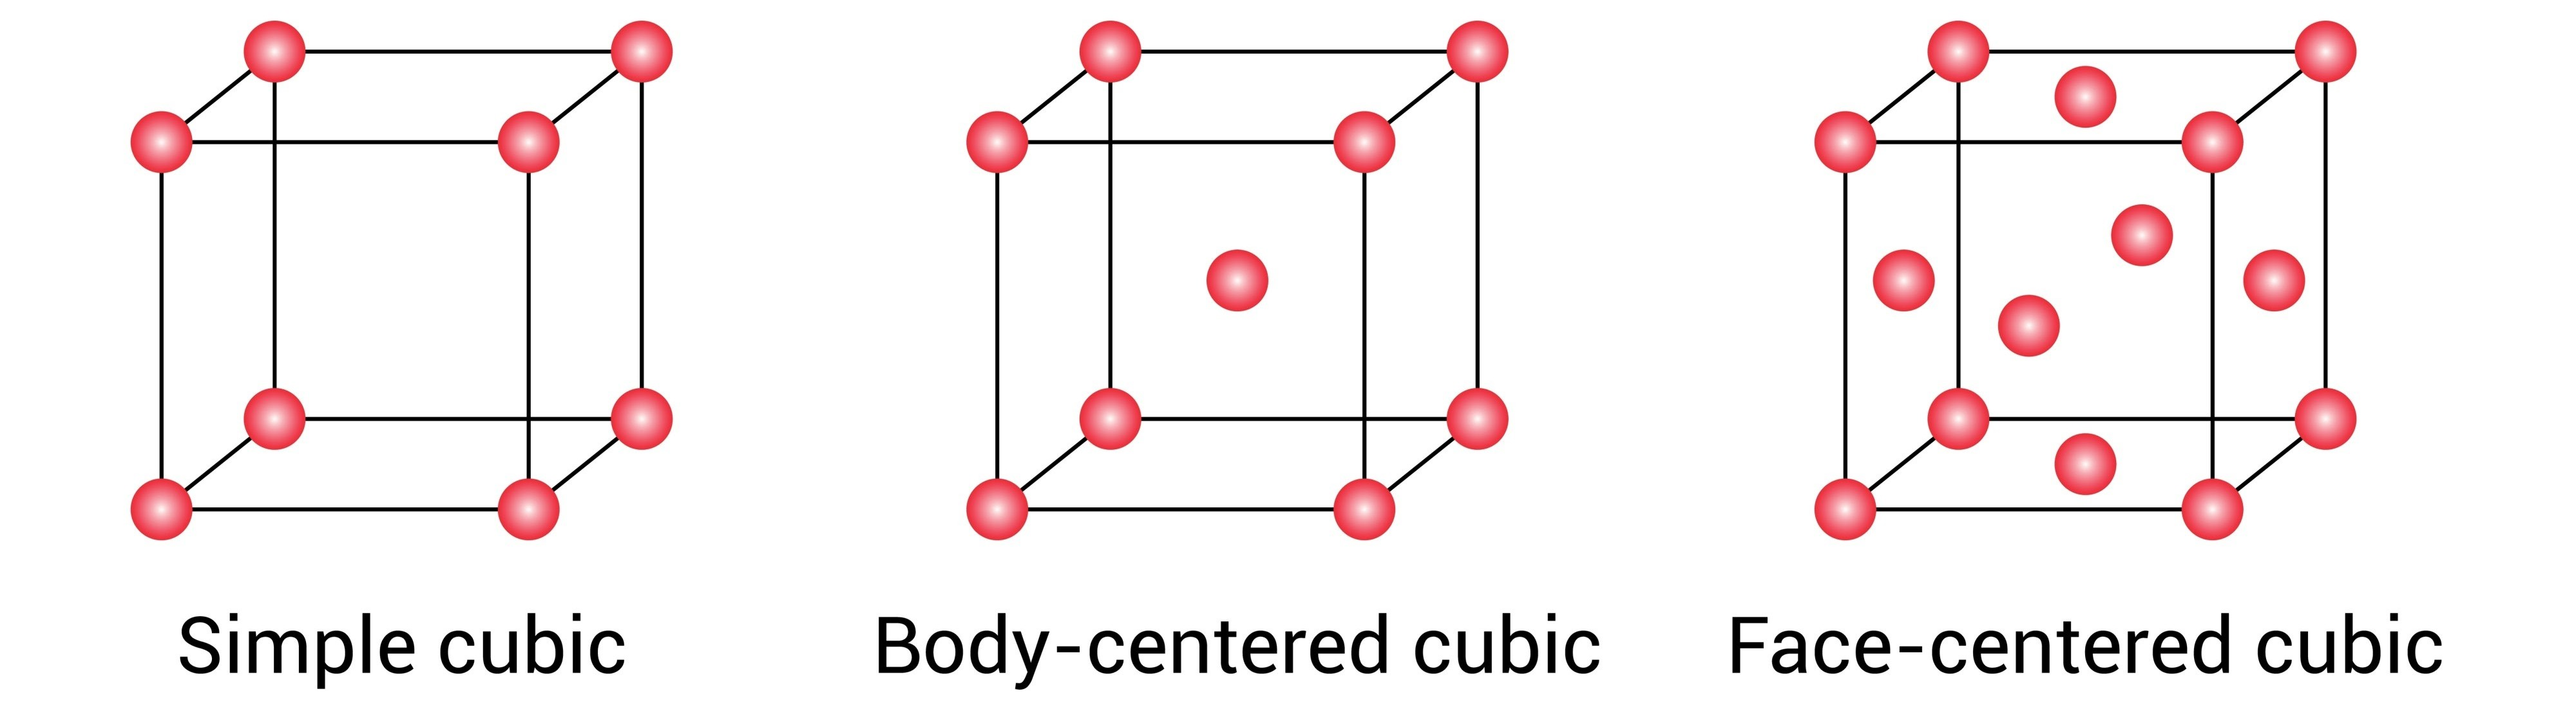
\includegraphics[width=0.9\linewidth]{cubicunitcells.jpg}
  \end{center}

  \subsection*{Coordinate Systems \& Miller Indices}
  \textbf{Points:} \( q \ r \ s \) (fractional multiples of edge lengths). \\
  \textbf{Directions:} \( [u \ v \ w] \) (Head coord. - Tail coord., clear fractions).\\
  \textbf{Planes (Miller Indices):}
  1. If plane passes through origin, establish new origin.
  2. Find intercepts on \( x, y, z \) axes (parallel = \( \infty \)).
  3. Take reciprocals of intercepts.
  4. Multiply to clear fractions (smallest integers).
  5. Enclose in parentheses \( (hkl) \). Negative intercepts get a bar (e.g., \( \bar{1} \)).

  \subsection*{Concepts}
  \textbf{Crystalline vs. Amorphous:} Crystalline has long-range order; amorphous lacks it. \\
  \textbf{Isotropy/Anisotropy:} Isotropic properties are independent of direction; anisotropic vary.

  \section*{Chapter 4: Imperfections in Solids}
  \subsection*{Concepts}
  \textbf{Vacancy Defect:} A point defect where an atom is missing from its normal structural lattice site. \\
  \textbf{Self-Interstitial Defect:} A point defect where an extra atom from the crystal is crowded into an interstitial void space that is normally empty.

  \subsection*{Key Equations}
  \textbf{Total Atomic Sites:} \( N = \frac{N_{A} \rho}{A} \) \\
  (\( N \): total atomic sites per volume, \( \rho \): density)\\

  \textbf{Equilibrium Vacancies:} \( N_{v} = N \exp\left(-\frac{Q_{v}}{kT}\right) \) \\
  (\( N_{v} \): number of vacancies, \( Q_{v} \): activation energy for vacancy formation)\\
  Constant: \( k = 8.62 \times 10^{-5} \text{ eV/atom}\cdot\text{K} \). (\( T \): temp in Kelvin). \\

  \textbf{Mass to Weight \%:} \( C_{1} = \frac{m_{1}}{m_{1} + m_{2}} \times 100 \) \\

  \textbf{Weight \% to Atom \%:} \\
  \( C'_{1} = \frac{C_{1} / A_{1}}{C_{1} / A_{1} + C_{2} / A_{2}} \times 100 \) \\
  (\( C'_{1} \): atom percent of element 1, \( A_{1}, A_{2} \): atomic weights) \\

  \textbf{Atom \% to Weight \%:} \\
  \( C_{1} = \frac{C'_{1} A_{1}}{C'_{1} A_{1} + C'_{2} A_{2}} \times 100 \)  \\
  (\( C_{1} \): weight percent of element 1)

  \subsection*{Example: Equilibrium Vacancies}
  Gold at \( 900^\circ\text{C} \) (\( 1173 \) K), \( Q_v = 0.98 \) eV/atom, \( A = 196.9 \) g/mol, \( \rho = 18.63 \times 10^6 \text{ g/m}^3 \). \\
  \( N = \frac{(6.022 \times 10^{23})(18.63 \times 10^{6})}{196.9} = 5.70 \times 10^{28} \text{ atoms/m}^3 \). \\
  \( N_v = (5.70 \times 10^{28}) \exp\left(-\frac{0.98}{(8.62 \times 10^{-5})(1173)}\right) \\ = 3.52 \times 10^{24} \text{ vacancies/m}^3 \)

\end{multicols*}
\end{document}
